% !TeX root = RJwrapper.tex
\title{An R-Squared for Multivariate Outcomes}
\author{by Tommy Jones and Mark J. Meyer}

\maketitle

\abstract{%
An abstract of less than 150 words.
}

\hypertarget{introduction}{%
\subsection{Introduction}\label{introduction}}

Introductory section which may include references in parentheses
\citep{R}, or cite a reference such as \citet{R} in the text.

\hypertarget{a-geometric-interpretation-of-r2}{%
\subsection{\texorpdfstring{A geometric interpretation of
\(R^2\)}{A geometric interpretation of R\^{}2}}\label{a-geometric-interpretation-of-r2}}

This section may contain a figure such as Figure \ref{fig:Rlogo}.

\begin{Schunk}
\begin{figure}[htbp]

{\centering 
\includegraphics[width=2in]{Rlogo-5} 

}

\caption[The logo of R]{The logo of R.}\label{fig:Rlogo}
\end{figure}
\end{Schunk}

\hypertarget{the-mvrsquared-package}{%
\subsection{\texorpdfstring{The \texttt{mvrsquared}
package}{The mvrsquared package}}\label{the-mvrsquared-package}}

There will likely be several sections, perhaps including code snippets,
such as:

\begin{Schunk}
\begin{Sinput}
x <- 1:10
plot(x)
\end{Sinput}

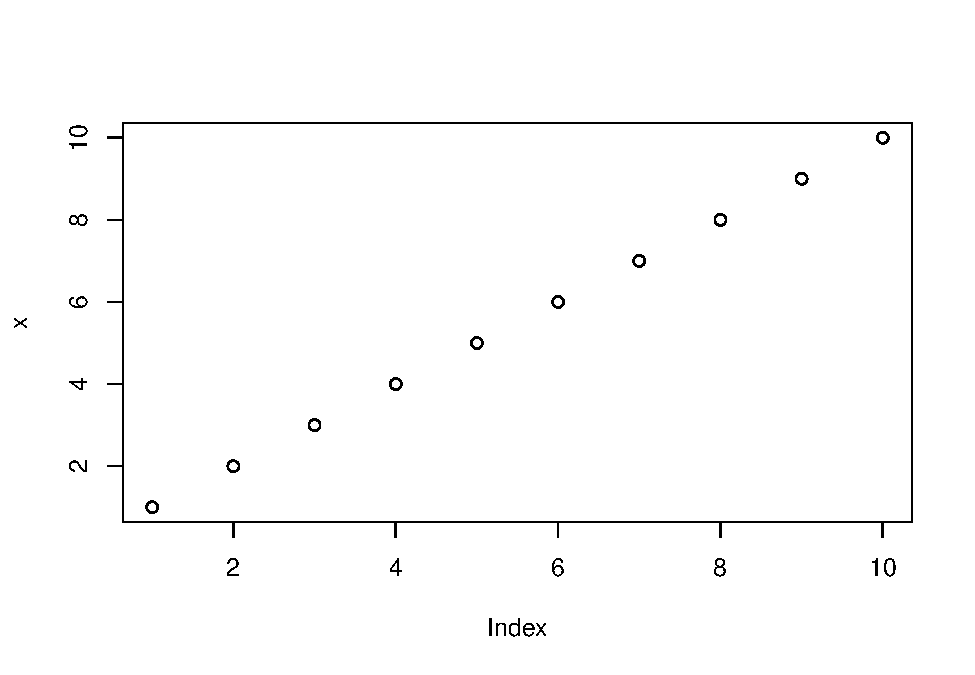
\includegraphics{Multivariate-R-Squared_files/figure-latex/unnamed-chunk-1-1} \end{Schunk}

\hypertarget{use-cases}{%
\subsection{Use cases}\label{use-cases}}

\hypertarget{r2-for-probabilistic-topic-models}{%
\subsubsection{\texorpdfstring{\(R^2\) for probabilistic topic
models}{R\^{}2 for probabilistic topic models}}\label{r2-for-probabilistic-topic-models}}

\hypertarget{second-use-case}{%
\subsubsection{Second use case}\label{second-use-case}}

\hypertarget{third-use-case}{%
\subsubsection{Third use case}\label{third-use-case}}

\hypertarget{summary}{%
\subsection{Summary}\label{summary}}

This file is only a basic article template. For full details of
\emph{The R Journal} style and information on how to prepare your
article for submission, see the
\href{https://journal.r-project.org/share/author-guide.pdf}{Instructions
for Authors}.

\hypertarget{about-this-format-and-the-r-journal-requirements}{%
\subsubsection{About this format and the R Journal
requirements}\label{about-this-format-and-the-r-journal-requirements}}

\texttt{rticles::rjournal\_article} will help you build the correct
files requirements:

\begin{itemize}
\tightlist
\item
  A R file will be generated automatically using \texttt{knitr::purl} -
  see \url{https://bookdown.org/yihui/rmarkdown-cookbook/purl.html} for
  more information.
\item
  A tex file will be generated from this Rmd file and correctly included
  in \texttt{RJwapper.tex} as expected to build \texttt{RJwrapper.pdf}.
\item
  All figure files will be kept in the default rmarkdown
  \texttt{*\_files} folder. This happens because
  \texttt{keep\_tex\ =\ TRUE} by default in
  \texttt{rticles::rjournal\_article}
\item
  Only the bib filename is to modifed. An example bib file is included
  in the template (\texttt{RJreferences.bib}) and you will have to name
  your bib file as the tex, R, and pdf files.
\end{itemize}

\bibliography{Multivariate-R-Squared.bib}

\address{%
Tommy Jones\\
Foundation\\%
1600 N Quinn St.~APT 202\\ Arlington, VA 22209\\
%
\url{https://journal.r-project.org}\\%
\textit{ORCiD: \href{https://orcid.org/0000-0001-6457-2452}{0000-0001-6457-2452}}\\%
\href{mailto:tommy@foundatn.com}{\nolinkurl{tommy@foundatn.com}}%
}

\address{%
Mark J. Meyer\\
Georgetown University\\%
3700 O St NW\\ Washington, DC 20057\\
%
\url{https://journal.r-project.org}\\%
\textit{ORCiD: \href{https://orcid.org/0000-0003-3942-9675}{0000-0003-3942-9675}}\\%
\href{mailto:mjm556@georgetown.edu}{\nolinkurl{mjm556@georgetown.edu}}%
}
